\documentclass[solution, letterpaper]{cs121}

\usepackage{tikz-qtree}
\usepackage{graphicx}
\usepackage{amsmath}

\DeclareMathOperator*{\argmax}{\arg\!\max}

%% Please fill in your name and collaboration statement here.
%\newcommand{\studentName}{Renzo Lucioni and Daniel Broudy}
%\newcommand{\collaborationStatement}{I collaborated with...}
\newcommand{\solncolor}{red}
\begin{document}

\header{5}{April 26, 2013, at 12:00 PM}{}{}

%%%%%%%%%%%%%%%%%%%%%%%%%%%%%%%%%%%%%%%%%%%%%%%%%%%%
\problem{10} %1

\subproblem{} %a
In this problem, our team decides to use a decision theoretic (i.e., greedy) strategy to decide where the dart thrower should aim. We have access to a probability distribution $P$ over the $N$ possible results of a dart throw, given a target $a \in A$, where $A$ is a finite set of targets. We also have access to a utility function $U$ which specifies the value to us of a dart throw result given our current score, which we denote with the random variable $S = s$. For clarity, note that a dart throw result is a certain number of points, and the utility is the \emph{value to us} of that dart throw result. We represent the result of a dart throw aimed at target $a$ with the random variable $R(a) = r_n(a)$, for all $n \in N$. The following equations determine $a^*$, the optimal action given the current score $s$, by adhering to the maximum expected utility (MEU) principle and choosing the action which maximizes the expected utility.

\begin{eqnarray}
\mathbb{E}\left[U(R(a),S)\right] = \sum_{n=1}^N P(r_n(a) | a) U(r_n(a),s) \\
a^* = \argmax_{a \in A} \mathbb{E}\left[U(R(a),S)\right] = \argmax_{a \in A} \sum_{n=1}^N P(r_n(a) | a) U(r_n(a),s)
\end{eqnarray}

\subproblem{} %b
Since the proposed utility function dictates a greedy approach, always preferring larger score reductions to smaller ones, we think the proposed utility function is useful only in a setting where long-term planning is not required. The game of ``301" requires greedy, short-term planning in the early game, where it is best to rack up points quickly, as well as long-term planning in the mid to late game, where it is best to recalculate your ``out" number sequences after each throw in an effort to end the game (i.e., get to 0) as quickly as possible. Note that the latter rarely involves consistently shooting for the largest point values, but instead shooting for a series of smaller numbers which sum to the current score.

A dart player designed using the greedy proposal will only consider the reward for the next, most immediate throw. With the above in mind, we would expect this dart player to make good decisions in the early game, preferring the largest point values it can achieve in an effort to ``get in" (i.e., lower the score) quickly. However, we would expect this dart player to make poor decisions in the mid to late game, since it would be unable to sacrifice short-term gain (i.e., choosing smaller point values) for long-term benefit (i.e., winning the game), continuing to select the largest valued throws possible instead of attempting to string together a series of lesser valued but smarter throws.


\problem{28} %2

\subproblem{} %a
The \textsc{START\_SCORE}+1 possible game scores in the range [0,\textsc{START\_SCORE}] constitute the states of our MDP model. Meanwhile, each possible (throw at a) \emph{target} on the dartboard constitutes an action in our MDP model.

\subproblem{} %b
Our reward function awards 0 reward to dart throw results (i.e., number of points) over the current score. Dart throw results under the current score are awarded reward equal to their point value. The discount factor, $\gamma$, plays no role in defining our reward function.

\subproblem{} %c
(See {\tt mdp.py} for the completed transition function.)

\subproblem{} %d
We choose to use an infinite rather than finite horizon when finding an optimal policy in the darts scenario because we know that the dart throwing agent will die at some point (i.e., win the game), but we do not have an upper bound on how long it will take for it to end the game and die. In this case, it is possible, albeit extremely unlikely, for the agent to go on living forever, with the game never ending. As such, the agent's total reward might be unbounded, so the problem of maximizing the total reward in a finite number of steps is ill-posed.

\subproblem{} %e
After uncommenting print statements which listed the optimal target given the current state for all states, it appears that the intuition behind the optimal policy resulting from value iteration using the small game is to go for the largest possible point value given the current score in the safest manner possible. That is, in each state (i.e., score) the agent chooses a point value which will get it as close as possible to ending the game. If there are multiple ways to achieve this point value, it seems that the agent chooses the method which will still allow it to make a dent in the score if it misses, as opposed to risking point value higher than the score, in which case the score does not decrease.

\subproblem{} %f
As the discount factor $\gamma$ approaches 1, the agent's optimal policy becomes less intent on winning the game immediately, trying for point values which are not necessarily the largest possible, given the score. When $\gamma \geq 1$, the agent attempts to live forever by always aiming for a miss, since this allows it to accumulate substantial reward indefinitely. When $\gamma$ approaches 0, the agent's optimal policy attempts to end the game as quickly as possible by trying for the largest point values possible, given the score. It seems that the range $0 \leq \gamma \leq 0.5$ is the sweet spot for creating this strictly greedy behavior. Common across all optimal policies are an apparent preference for the outer ring of the board, as well as the fact that the game eventually ends.

\problem{25} %3

\subproblem{} %a
DANBRO

\subproblem{} %b
DANBRO

\subproblem{} %c
By (A), we know that if policy iteration terminates, it terminates with the optimal stationary policy. By (B), we know that the policy improves or stays that same after each iteration phase (i.e., every step the policy improves). This means that a given policy can be encountered at most once. Since there are a finite number of states and actions, there are a finite number of policies. Therefore, we must terminate by the time we have iterated through the finite number of policies. Assuming the policy space is convex, we can hence say that policy iteration always terminates with an optimal stationary policy.


\problem{30} %4

\subproblem{} %a
We implemented time-$T$ mode switching and $\varepsilon$-Greedy strategies for balancing exploration and exploitation. See {\tt modelbased.py} for our implementations. The following graphs, one for each exploration/exploitation strategy, show the relationship between performance (average number of throws to complete a game) and epoch size used to update the optimal policy.

\begin{center}
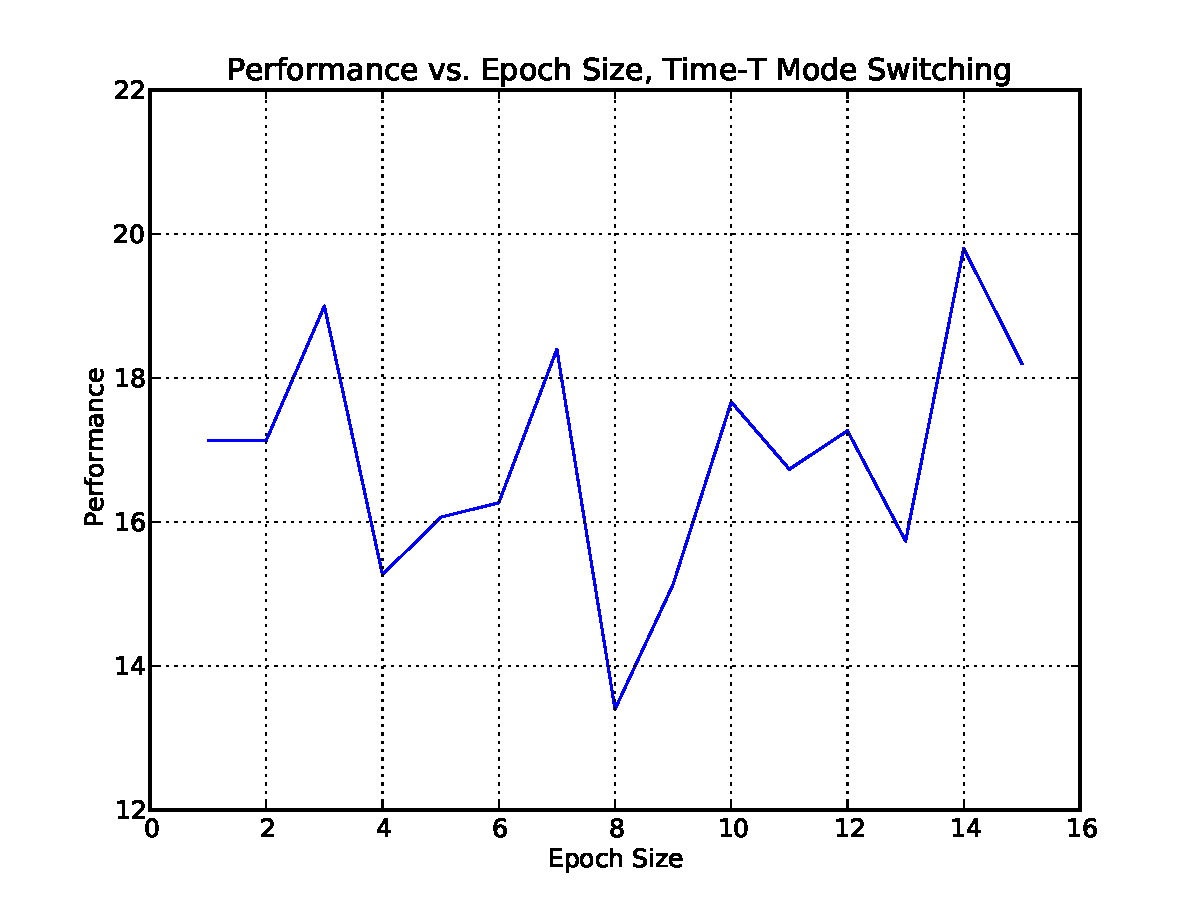
\includegraphics[scale=0.8]{source/perf-v-epoch-mode-switch.pdf}
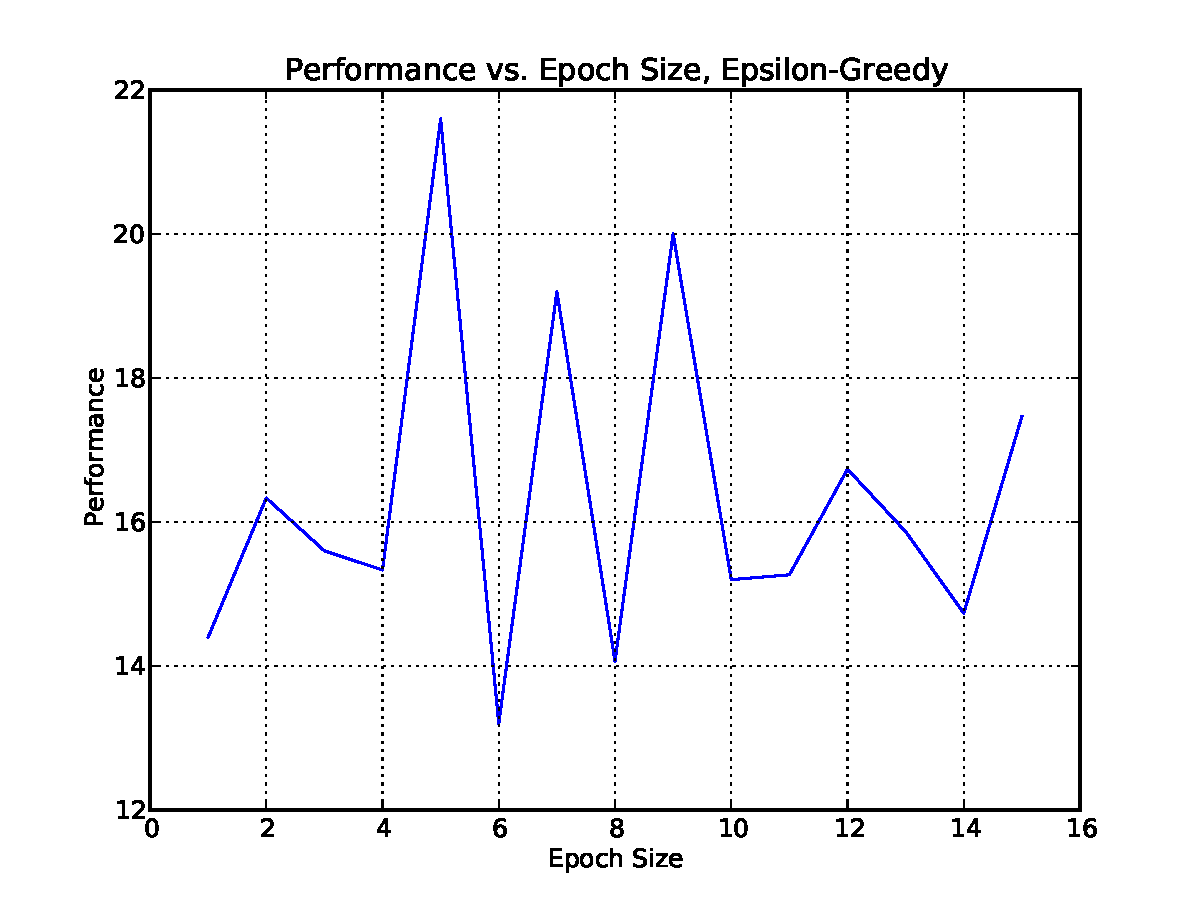
\includegraphics[scale=0.8]{source/perf-v-epoch-greedy.pdf}
\end{center}

\emph{How are performance and epoch size related? How do the two strategies compare? It's hard to tell with these noisy graphs.}

\subproblem{} %b
DANBRO

\subproblem{} %c
DANBRO



\end{document}